\documentclass[12pt,twoside]{book}
\usepackage[a4paper,inner=3.5cm,outer=2.5cm,top=2.5cm,bottom=2.5cm]{geometry}
\usepackage{fontspec}
\usepackage{polski}
\usepackage[polish]{babel}
\setmainfont{Times New Roman}
\usepackage{setspace}
\setstretch{1.5}
\usepackage{fancyhdr}
\pagestyle{fancy}
\fancyhf{}
\fancyfoot[CE,CO]{\thepage}
\renewcommand{\headrulewidth}{0pt}
\fancypagestyle{plain}{%
  \fancyhf{}%
  \renewcommand{\headrulewidth}{0pt}%
  \fancyfoot[CE,CO]{\thepage}%
}

% Formatting
\usepackage{titlesec}

% Konfiguracja nagłówków
% Nagłówek 1. stopnia: 12 pkt, WERSALIKI, pogrubiona
\titleformat{\chapter}[hang]
  {\normalfont\bfseries\fontsize{12}{14}\selectfont\uppercase}
  {\thechapter.}
  {1em}
  {}
  
% Nagłówek 2. stopnia: 10 pkt, pogrubiona i kursywa
\titleformat{\section}
  {\normalfont\bfseries\itshape\fontsize{10}{12}\selectfont}
  {\thesection}
  {1em}
  {}

% Nagłówek 3. stopnia: 10 pkt, kursywa
\titleformat{\subsection}
  {\normalfont\itshape\fontsize{10}{12}\selectfont}
  {\thesubsection}
  {1em}
  {}

% Dostosowanie odstępów dla nagłówków
\titlespacing*{\chapter}{0pt}{12pt}{6pt}
\titlespacing*{\section}{0pt}{12pt}{6pt}
\titlespacing*{\subsection}{0pt}{12pt}{6pt}

\usepackage{lipsum}
\usepackage{pdfpages}
\usepackage{tocloft}
\usepackage{cite}
\usepackage{indentfirst}

\renewcommand{\contentsname}{Spis treści}
\renewcommand{\cftchapleader}{\cftdotfill{\cftdotsep}}
\renewcommand{\cfttoctitlefont}{\bfseries\fontsize{12pt}{14pt}\selectfont}
\renewcommand{\cftloftitlefont}{\bfseries\fontsize{12pt}{14pt}\selectfont}

\setlength{\parindent}{1.25cm}

\usepackage{graphicx}
\usepackage[font=normalsize,labelfont=bf]{caption} % Konfiguracja podpisów

\captionsetup[figure]{
  labelsep=period, % Ustawienie kropki zamiast dwukropka
  justification=centering, % Wyśrodkowanie podpisu
  font=normalsize, % Rozmiar czcionki podpisu
  textfont=normalfont, % Styl czcionki podpisu
  labelfont=normalfont, % Pogrubienie etykiety "Rys."
  name=Rys. % Zmiana nazwy "Rysunek" na "Rys."
}

\begin{document}

\setcounter{page}{1}
\thispagestyle{empty}
\includepdf{includes/pdf/strona_tytułowa.pdf}

% Tutaj umieść swoją stronę ze spisem treści
\tableofcontents

% Tutaj zaczyna się główna treść pracy
\chapter{Wstęp}

\section{Cel pracy}

Celem niniejszej pracy dyplomowej jest zbadanie procesu migracji systemu monolitycznego do architektury mikroserwisowej opartej o usługi chmury obliczeniowej dostawcy Amazon Web Services (w skrócie AWS) pod kątem ulepszenia zabezpieczeń omawianego systemu. System objęty badaniem, to: „System do internetowego wspomagania pacjenta i lekarza”, który został w całości zaprojektowany i zaimplementowany w formie monolitycznej przez autora pracy dyplomowej jako projekt inżynierski w celu ukończenia studiów inżynierskich pierwszego stopnia. Wybór systemu do przeprowadzenia analizy motywowany jest znajomością jego architektury, wpasowującą się doskonale w temat pracy oraz motywacja do jego dalszego rozwijania i ulepszania w zakresie cyberbezpieczeństwa.

Analiza procesu migracji oraz rozwinięcia systemu zabezpieczeń systemu ma wykazać jak dobrze usługi chmurowe ochraniają swoich usługobiorców i ich oprogramowania przed popularnymi atakami hakerskimi oraz jak duży wpływ na bezpieczeństwo systemu ma jego architektura. Narzędzia używane przez autor pracy to przede wszystkim oprogramowanie wirtualizujące systemy operacyjne Docker, język programowania PHP, język programowania Java Script, zestaw narzędzi programistycznych Symfony oraz Vue.js, dodatkowo usługi AWS, takie jak: Elastic Compute Cloud (w skrócie EC2), Relational Databases (w skrócie RDS), Route 53, Code Pipeline, Code Build, Code Deploy, Elastic Cache, Simple Storage Service, Elastic Container Registry, Lambda. Również narzędzia do analizy ruchu sieciowego, takie jak: Wireshark.

Praca ta omówia aspekty takie jak: ewaluacja zastanej architektury aplikacji, planowanie architektury mikroserwisowej w chmurze AWS, ocena zagadnień bezpieczeństwa podczas migracji, implementacja i wdrażanie mikroserwisów w chmurze AWS, ocena i analiza wyników. Każdy wymieniony etap pracy jest szczegółowo omówiony, odzwierciedlając wiedzę i doświadczenie akademickie jak i zawodowe autora.

\section{Motywacja}

Motywacją do podjęcia tematu pracy są doświadczenia autora na tle zawodowym, które przyspieszyły naukę w zakresie obliczeń chmurowych. Jednak największym motywatorem do wykonania badania jest kontynuacja pracy akademickiej, dążenie do ciągłego rozwoju wyprodukowanego przez siebie oprogramowania i wdrażanie wiedzy pozyskanej w czasie studiów drugiego stopnia, tak by umiejętnie zabezpieczać oprogramowanie. Dodatkowym motywatorem jest również fakt, iż technologia chmurowa każdego roku zdobywa coraz większy udział na rynku usług hostingowych, a także staje się dzięki wzrastającej konkurencyjności przystępniejsza dla mniejszych firm lub prywatnych odbiorców. Serwis Precedence Research przewiduje, iż w nadchodzących ośmiu latach udział rynkowy technologii chmurowych zwiększy się około pięciokrotnie do wartości 2297 miliardów dolarów \cite{p.research}. Patrz Rysunek~\ref{fig:precedence-research}.

\begin{figure}[ht]
\centering
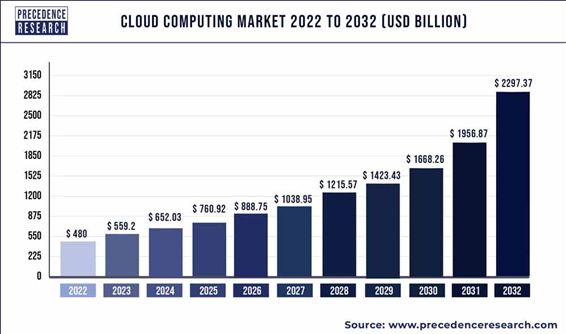
\includegraphics[width=\textwidth]{includes/images/precedence-research.png}
\caption{Wykres przedstawiający prognozę wzrostu udziału rynkowego technologii chmurowej}
\label{fig:precedence-research}
\end{figure}

\section{Założenia i spodziewane wyniki}

Rezultatem niniejszej pracy dyplomowej jest rozebranie monolitycznego systemu na mikroserwisy z pojedynczą odpowiedzialnością logiczną. Zasada działa aplikacji nie ulega zmianie, dla użytkownika zewnętrznego wprowadzenie zmiany powinno odbyć się bez odczuwalnej różnicy. Samo rozczłonkowanie systemu odbywa jak najbardziej atomicznie się da przy rozsądnym nakłądzie pracy pozwalającym ukończyć tę pracę w terminie jej obrony. Autor zakłada, iż poprawie ulegnie bezpieczeństwo danych przechowywanych w bazie danych poprzez ukrycie bazy danych przed dostępem z zewnątrz przy wykorzystaniu wirtualnej sieci prywatnej, także większa granularność aplikacji poprawi bezpieczeństwo wdrożenia zmian poprzez ustystematyzowanie procesu jaki za tym stoi poprzez wykorzystanie technologii „Pipeline” (ciąg zautomatyzowanych procesów dostarczania nowego oprogramowania). Również autor odświeżył wersję zależności z jakich składa się projekt, tak by rozwiązać problemy luk bezpieczeństwa wynikających z użycia przestarzałych bibliotek. Dodatkowym poziomem ulepszenia zabezpieczeń aplikacji będzie przeszukanie kodu w pod kątem znalezienia luk logicznych lub twardo zakodowanych dostępów, takich jak hasła do bazy danych lub inne, z których aplikacja korzysta.

\chapter{Ewaluacja zastanej architektury aplikacji}

Zgodnie z stanem aplikacji z dnia 11.06.2022r. projekt “System do internetowego wspomagania pacjenta i lekarza” oparty jest o kilka składowych jakie należy wyróżnić, a są nimi:

\begin{itemize}
\item Baza danych oprata o silnik MySQL.
\item Trzon logiki biznesowej oparty o zestaw narzędzi Symfony w wersji 5.4.
\item Warstwa widoku aplikacji oparta o silnik Twig oraz Vue.js.
\item Silnik nginx jako narzędzie do przekazania zapytania klienckiego do logiki biznesowej.
\end{itemize}

Wyróżnione komponenty są ściśle ze sobą połączone. Logika biznesowa oraz baza danych są nierozerwalne, logika biznesowa posiada klasy encji, które bezpośrednio przekładają się na tabele w bazie danych. Logika biznesowa również decyduje o tym jaki widok jest obecnie wyświetlany, a warstwa widoku bazuje na tym, co dostarczył kontroler Symfony. Cały zestaw wykorzystuje narzędzie nginx do tego, by otrzymać zapytanie od klienta. W niniejszym rodziale zostaną przedstawione kolejno wyżej wymienione komponenty z szerszym opisem co do każdego z nich.

\section{Logika biznesowa i baza danych}

Symfony jako framework, który za zadanie ma ułatwić rozwój oprogramowania internetowego w projekcie z pracy inżynierskiej autora niniejszej pracy spełnił swoją rolę niejako przyczyniając się do skrócenia czasu potrzebnego na rzecz implementacji założeń diagramów użyć, odwzwierciedlenie domen każdego z aktorów systemu, a także diagramów przepływu danych. Narzędzia takie jak wbudowane kontrolery z dostępnym API do zapytań, czy formularze do walidacji danych wejściowych do systemu, router odpowiadający na zapytania, czy szablony wspierane przez silnik Twig to tylko niektóre z narzędzi jakie zostały wykorzystane przy okazji implementacji. Wyczerpujący schemat udogodnień oferowanych przez Symfony znajduje się na Rysunku~\ref{fig:symfony-metadata-scheme}.

\begin{figure}[ht]
\centering
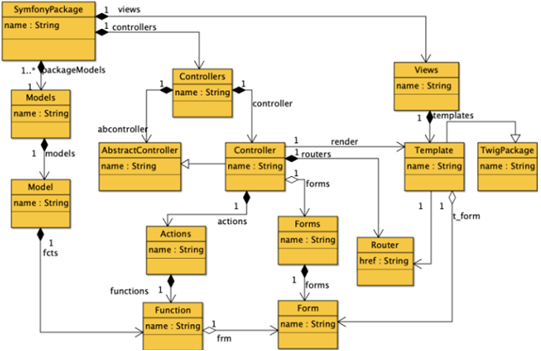
\includegraphics[width=\textwidth]{includes/images/symfony-metadata-scheme.png}
\caption{Schemat metamodelu Symfony \cite{mod.driv.arch.symf}}
\label{fig:symfony-metadata-scheme}
\end{figure}

W celu odzwierciedlenia domen aktorów, w projekcie została wykorzystana biblioteka Doctrine, wspierana przez Symfony. Samo Doctrine to narzędzie do maniplacji bazą danych przy wykorzystaniu obiektów PHP \cite{symf.5}.

\bibliographystyle{IEEEtran}
\bibliography{bibliography.bib}
\listoffigures
\end{document}
